% Week 10 evidence: tables and figures read the CSV files one level up.
% Compile: cd evidence/week10/latex && xelatex main.tex   (or lualatex; needs fontspec)
% In the thesis: \usepackage{pgfplots,booktabs}, \pgfplotsset{compat=1.17},
% \usepgfplotslibrary{groupplots,statistics,fillbetween}, \newcommand{\evdir}{<path to evidence/week10>}
% then \input{<path>/fig9_gradual_timeline.tex} etc.
\documentclass[11pt]{article}
\usepackage{fontspec}
\usepackage[a4paper,margin=2cm]{geometry}
\usepackage{booktabs,float,caption}
\usepackage{pgfplots,pgfplotstable}
\pgfplotsset{compat=1.17}
\usepgfplotslibrary{groupplots,statistics,fillbetween}
\newcommand{\evdir}{..}
\pgfplotsset{every axis/.append style={font=\small},
  w10/.style={width=0.95\linewidth,height=5cm,grid=major,grid style={gray!25}}}
\begin{document}
\section*{Tuần 10 -- Bảng và hình từ evidence/week10}
\begin{table}[H]\centering\small
\caption{Thống kê dataset (mẫu hợp lệ)}\label{tab:w10-dataset}
\begin{tabular}{lrrrrrrrr}\toprule
Biến & n & mean & std & min & median & p95 & max & missing \% \\\midrule
utilization & 9000 & 0.687 & 0.171 & 0.056 & 0.659 & 0.935 & 1.103 & 0.000 \\
processed\_packet\_in\_rate & 9000 & 984.218 & 245.093 & 80.929 & 944.370 & 1339.576 & 1580.000 & 0.000 \\
flow\_mod\_rate & 9000 & 965.110 & 258.679 & 0.000 & 901.397 & 1333.240 & 1580.000 & 0.000 \\
process\_cpu\_percent & 9000 & 75.212 & 11.230 & 11.000 & 73.900 & 90.900 & 98.900 & 0.000 \\
process\_memory\_rss\_mb & 9000 & 56.852 & 0.203 & 56.648 & 56.852 & 57.055 & 57.055 & 0.000 \\
response\_p95\_ms & 9000 & 0.735 & 0.087 & 0.396 & 0.766 & 0.828 & 1.346 & 0.000 \\
max\_switch\_control\_load\_share & 9000 & 0.189 & 0.177 & 0.100 & 0.101 & 0.550 & 0.567 & 0.000 \\
age\_of\_twin\_ms & 9000 & 769.932 & 146.064 & 449.076 & 775.361 & 991.169 & 1024.503 & 0.000 \\
completeness\_ratio & 9000 & 1.000 & 0.000 & 1.000 & 1.000 & 1.000 & 1.000 & 0.000 \\
synchronization\_jitter\_ms & 9000 & 508.981 & 48.825 & 400.488 & 484.982 & 576.171 & 602.282 & 0.000 \\
\bottomrule\end{tabular}
\end{table}


\begin{table}[H]\centering\small
\caption{Horizon v1: $T_{detect}+T_{decision}+T_{migrate}\le h$}\label{tab:w10-horizon}
\begin{tabular}{lr}\toprule
Thành phần & ms \\\midrule
$T_{detect}$ (P95 thu telemetry) & 568.579 \\
$T_{decision}$ (suy luận + bước dự báo) & 4.682 \\
$T_{migrate}$ (P95 migration) & 2132.906 \\
Ngân sách cho quyết định & 298.515 \\
Dư & 293.833 \\
\bottomrule\end{tabular}
\end{table}


\begin{table}[H]\centering\small
\caption{Năm mô hình trên Test}\label{tab:w10-test}
\begin{tabular}{lrrrrr}\toprule
Model & MAE & RMSE & MAPE (\%) & $R^2$ & P95 $|e|$ \\\midrule
persistence & 0.0494 & 0.0980 & 7.5186 & 0.7046 & 0.1780 \\
moving\_average\_w3 & 0.0595 & 0.1147 & 9.0688 & 0.5950 & 0.2282 \\
linear\_regression & 0.0369 & 0.0698 & 5.7666 & 0.8502 & 0.1306 \\
random\_forest & 0.0152 & 0.0424 & 2.3108 & 0.9446 & 0.0512 \\
xgboost & 0.0150 & 0.0409 & 2.3412 & 0.9486 & 0.0431 \\
\bottomrule\end{tabular}
\end{table}


\begin{table}[H]\centering\small
\caption{Chọn mô hình trên Validation ($S_m$ nhỏ hơn là tốt hơn)}\label{tab:w10-selection}
\begin{tabular}{llrrrrr}\toprule
Hạng & Model & RMSE & P95 $|e|$ & RMSE/Persistence & P95 latency (ms) & $S_m$ \\\midrule
1 & xgboost & 0.0385 & 0.0513 & 0.3879 & 0.5046 & 0.3074 \\
2 & random\_forest & 0.0426 & 0.0545 & 0.4287 & 32.6800 & 0.3378 \\
3 & linear\_regression & 0.0700 & 0.1309 & 0.7045 & 0.1553 & 0.6477 \\
4 & persistence & 0.0993 & 0.1804 & 1.0000 & 0.0005 & 0.9000 \\
5 & moving\_average\_w3 & 0.1158 & 0.2286 & 1.1666 & 0.0115 & 1.0859 \\
\bottomrule\end{tabular}
\end{table}


\begin{table}[H]\centering\small
\caption{Độ nhạy Quality Score theo bộ trọng số}\label{tab:w10-quality}
\begin{tabular}{lrrrrrrr}\toprule
Biến thể & mean & min & max $|\Delta|$ & Spearman & Kendall & valid & eligible \\\midrule
base & 0.972 & 0.680 & 0.000 & 1.000 & 1.000 & 693 & 693 \\
consistency\_heavy & 0.972 & 0.680 & 0.003 & 1.000 & 1.000 & 693 & 693 \\
completeness\_heavy & 0.972 & 0.680 & 0.002 & 1.000 & 1.000 & 693 & 693 \\
freshness\_heavy & 0.971 & 0.630 & 0.050 & 1.000 & 1.000 & 693 & 693 \\
\bottomrule\end{tabular}
\end{table}


\begin{table}[H]\centering\small
\caption{Kịch bản runtime (khung workload)}\label{tab:w10-runtime}
\begin{tabular}{lrrrrrrrrr}\toprule
Kịch bản & READY & OOD & RMSE & RMSE pers. & Coverage & Quá tải & Báo trúng & Hụt & Nhầm \\\midrule
stable & 0.945 & 0.070 & 0.014 & 0.019 & 0.997 & 0 & 0 & 0 & 0 \\
gradual & 0.945 & 0.038 & 0.029 & 0.039 & 0.967 & 2 & 2 & 0 & 24 \\
burst & 0.945 & 0.038 & 0.079 & 0.138 & 0.962 & 36 & 30 & 6 & 12 \\
invalid\_snapshot & 0.505 & 0.000 & 0.018 & 0.024 & 0.983 & 0 & 0 & 0 & 0 \\
hot\_switch & 0.946 & 0.989 & 0.077 & 0.076 & 0.950 & 0 & 0 & 0 & 0 \\
migration & 0.879 & 0.669 & 0.026 & 0.028 & 0.997 & 0 & 0 & 0 & 0 \\
\bottomrule\end{tabular}
\end{table}


\begin{figure}[H]\centering
\begin{tikzpicture}
\begin{groupplot}[group style={group size=2 by 2,horizontal sep=1.6cm,vertical sep=1.6cm},
  width=0.48\linewidth,height=4.2cm,ylabel={samples},grid=major,grid style={gray!25},ymin=0,
  xticklabel style={/pgf/number format/fixed},scaled x ticks=false]
\nextgroupplot[xlabel={utilization $U$}]
\addplot[fill=blue!30,draw=blue!60,const plot mark left] table[col sep=comma,x=left,y=count]{\evdir/hist_utilization.csv} \closedcycle;
\nextgroupplot[xlabel={processed Packet-In rate (pps)}]
\addplot[fill=blue!30,draw=blue!60,const plot mark left] table[col sep=comma,x=left,y=count]{\evdir/hist_processed_packet_in_rate.csv} \closedcycle;
\nextgroupplot[xlabel={CPU (\%)}]
\addplot[fill=blue!30,draw=blue!60,const plot mark left] table[col sep=comma,x=left,y=count]{\evdir/hist_process_cpu_percent.csv} \closedcycle;
\nextgroupplot[xlabel={response P95 (ms)}]
\addplot[fill=blue!30,draw=blue!60,const plot mark left] table[col sep=comma,x=left,y=count]{\evdir/hist_response_p95_ms.csv} \closedcycle;
\end{groupplot}
\end{tikzpicture}

\caption*{Hình 1. Phân bố các biến chính của dataset (mẫu hợp lệ).}
\end{figure}

\begin{figure}[H]\centering
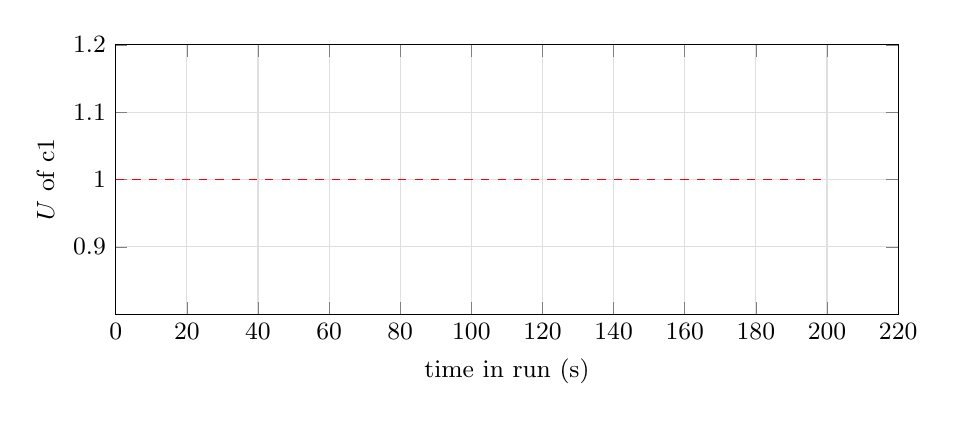
\begin{tikzpicture}
\begin{axis}[w10,xmin=0,xlabel={time in run (s)},ylabel={$U$ of c1},legend pos=outer north east,
  legend style={font=\scriptsize},cycle list name=color list]
\foreach \w/\n in {stable/stable,gradual/gradual,burst/burst,oscillating/oscillating,hot_switch/hot-switch}{
  \IfFileExists{\evdir/workload_profile_\w.csv}{
    \addplot+[no marks,thick] table[col sep=comma,x=t_s,y=utilization]{\evdir/workload_profile_\w.csv};
    \addlegendentryexpanded{\n}}{}}
\addplot[red,dashed,domain=0:200] {1.0};
\end{axis}
\end{tikzpicture}

\caption*{Hình 2. U(t) của năm workload (một run mỗi loại, controller c1).}
\end{figure}

\begin{figure}[H]\centering
\pgfplotstableread[col sep=comma]{\evdir/model_comparison_validation.csv}\val
\begin{tikzpicture}
\begin{axis}[w10,ybar,bar width=12pt,symbolic x coords={persistence,moving_average_w3,linear_regression,random_forest,xgboost},
  xtick={persistence,moving_average_w3,linear_regression,random_forest,xgboost},xticklabels={Persistence,MA(3),LR,RF,XGBoost},ylabel={validation RMSE},
  nodes near coords,nodes near coords style={font=\tiny,/pgf/number format/.cd,fixed,precision=3},ymin=0]
\addplot table[x=model,y=rmse]{\val};
\end{axis}
\end{tikzpicture}

\caption*{Hình 3. So sánh năm mô hình trên Validation (RMSE).}
\end{figure}

\begin{figure}[H]\centering
\pgfplotstableread[col sep=comma]{\evdir/model_comparison_test.csv}\tst
\begin{tikzpicture}
\begin{axis}[w10,ybar,bar width=10pt,symbolic x coords={persistence,moving_average_w3,linear_regression,random_forest,xgboost},
  xtick={persistence,moving_average_w3,linear_regression,random_forest,xgboost},xticklabels={Persistence,MA(3),LR,RF,XGBoost},ylabel={test error},legend pos=north east,ymin=0]
\addplot table[x=model,y=rmse]{\tst}; \addlegendentry{RMSE}
\addplot table[x=model,y=p95_absolute_error]{\tst}; \addlegendentry{P95 $|e|$}
\end{axis}
\end{tikzpicture}

\caption*{Hình 4. RMSE và P95 sai số tuyệt đối trên Test.}
\end{figure}

\begin{figure}[H]\centering
\pgfplotstableread[col sep=comma]{\evdir/per_workload_rmse_wide.csv}\pw
\begin{tikzpicture}
\begin{axis}[w10,ybar,bar width=5pt,symbolic x coords={stable,gradual,burst,oscillating,hot-switch},xtick={stable,gradual,burst,oscillating,hot-switch},
  ylabel={RMSE},legend style={font=\scriptsize,at={(0.5,-0.2)},anchor=north,legend columns=5},ymin=0]
\addplot table[x=workload,y=persistence]{\pw}; \addlegendentry{Persistence}
\addplot table[x=workload,y=moving_average_w3]{\pw}; \addlegendentry{MA(3)}
\addplot table[x=workload,y=linear_regression]{\pw}; \addlegendentry{LR}
\addplot table[x=workload,y=random_forest]{\pw}; \addlegendentry{RF}
\addplot table[x=workload,y=xgboost]{\pw}; \addlegendentry{XGBoost}
\end{axis}
\end{tikzpicture}

\caption*{Hình 5. RMSE theo workload (Test; hot-switch là Unseen).}
\end{figure}

\begin{figure}[H]\centering
\pgfplotstableread[col sep=comma]{\evdir/ood_degradation.csv}\ood
\begin{tikzpicture}
\begin{axis}[w10,ybar,bar width=10pt,symbolic x coords={validation,test,unseen},xtick={validation,test,unseen},
  xticklabels={Validation (ID),Test (ID),Hot-switch (OOD)},ylabel={RMSE},ymin=0,
  legend style={font=\scriptsize,at={(0.5,-0.22)},anchor=north,legend columns=3}]
\addplot table[x=split,y=rmse_without_gate]{\ood}; \addlegendentry{XGBoost, no gate}
\addplot table[x=split,y=rmse_with_gate]{\ood}; \addlegendentry{XGBoost + OOD gate}
\addplot table[x=split,y=rmse_persistence]{\ood}; \addlegendentry{Persistence}
\end{axis}
\end{tikzpicture}

\caption*{Hình 6. Test (ID) và Hot-switch (OOD): XGBoost có/không cổng OOD so với Persistence.}
\end{figure}

\begin{figure}[H]\centering
\pgfplotstableread[col sep=comma]{\evdir/inference_latency.csv}\lat
\begin{tikzpicture}
\begin{axis}[w10,ybar,bar width=12pt,ymode=log,log origin=infty,
  symbolic x coords={persistence,moving_average_w3,linear_regression,random_forest,xgboost},xtick={persistence,moving_average_w3,linear_regression,random_forest,xgboost},
  xticklabels={Persistence,MA(3),LR,RF,XGBoost},ylabel={single-sample P95 (ms, log)},legend pos=north west]
\addplot table[x=model,y=p95_ms]{\lat}; \addlegendentry{P95}
\addplot table[x=model,y=p50_ms]{\lat}; \addlegendentry{P50}
\end{axis}
\end{tikzpicture}

\caption*{Hình 7. Độ trễ suy luận một mẫu (P50, P95) khi testbed chạy.}
\end{figure}

\begin{figure}[H]\centering
\pgfplotstableread[col sep=comma]{\evdir/quality_sensitivity_invalid_snapshot.csv}\qs
\begin{tikzpicture}
\begin{axis}[w10,xlabel={time in run (s), telemetry-loss run},ylabel={Quality Score},ymin=0,ymax=1.05,
  legend style={font=\scriptsize,at={(0.5,-0.32)},anchor=north,legend columns=3}]
\addplot+[no marks,thick] table[x=t_s,y=base]{\qs}; \addlegendentry{base}
\addplot+[no marks] table[x=t_s,y=consistency_heavy]{\qs}; \addlegendentry{consistency-heavy}
\addplot+[no marks] table[x=t_s,y=completeness_heavy]{\qs}; \addlegendentry{completeness-heavy}
\addplot+[no marks] table[x=t_s,y=freshness_heavy]{\qs}; \addlegendentry{freshness-heavy}
\addplot[only marks,mark=|,red,mark size=2pt,unbounded coords=discard] table[x=t_s,y=invalid_mark]{\qs};
\addlegendentry{Hard Gate: invalid}
\end{axis}
\end{tikzpicture}

\caption*{Hình 8. Quality Score theo bốn bộ trọng số trên lượt mất telemetry; vạch đỏ: Hard Gate = invalid.}
\end{figure}

\begin{figure}[H]\centering
\begin{tikzpicture}
\begin{groupplot}[group style={group size=1 by 2,vertical sep=1.2cm},width=0.95\linewidth,height=5cm,
  grid=major,grid style={gray!25},unbounded coords=jump,ylabel={$U$},
  legend style={font=\scriptsize,at={(0.5,-0.32)},anchor=north,legend columns=4}]
\nextgroupplot[title={c1}]
\addplot[name path=hat,blue,thin] table[col sep=comma,x=t_target_s,y=u_hat]{\evdir/runtime_gradual_c1.csv};
\addplot[name path=up,draw=none,forget plot] table[col sep=comma,x=t_target_s,y=upper]{\evdir/runtime_gradual_c1.csv};
\addplot[blue!25,forget plot] fill between[of=hat and up];
\addplot[black,thick] table[col sep=comma,x=t_s,y=u]{\evdir/runtime_gradual_c1.csv};
\addplot[red,dashed,domain=0:200,forget plot] {1.0};
\addplot[only marks,red,mark=*,mark size=1.2pt] table[col sep=comma,x=t_target_s,y=alert_upper]{\evdir/runtime_gradual_c1.csv};
\addplot[only marks,orange,mark=x] table[col sep=comma,x=t_target_s,y=ood_u_hat]{\evdir/runtime_gradual_c1.csv};
\addplot[only marks,black,mark=triangle*] table[col sep=comma,x=t_s,y=measured_overload_u]{\evdir/runtime_gradual_c1.csv};
\nextgroupplot[title={c2},xlabel={seconds since workload start}]
\addplot[name path=hat2,blue,thin] table[col sep=comma,x=t_target_s,y=u_hat]{\evdir/runtime_gradual_c2.csv};
\addlegendentry{$\hat U$ at $t+h$}
\addplot[name path=up2,draw=none,forget plot] table[col sep=comma,x=t_target_s,y=upper]{\evdir/runtime_gradual_c2.csv};
\addplot[blue!25] fill between[of=hat2 and up2]; \addlegendentry{$+m_f$}
\addplot[black,thick] table[col sep=comma,x=t_s,y=u]{\evdir/runtime_gradual_c2.csv}; \addlegendentry{$U(t)$}
\addplot[red,dashed,domain=0:200] {1.0}; \addlegendentry{safe limit 1.0}
\addplot[only marks,red,mark=*,mark size=1.2pt] table[col sep=comma,x=t_target_s,y=alert_upper]{\evdir/runtime_gradual_c2.csv};
\addlegendentry{risk flag}
\addplot[only marks,orange,mark=x] table[col sep=comma,x=t_target_s,y=ood_u_hat]{\evdir/runtime_gradual_c2.csv};
\addlegendentry{OOD fallback}
\addplot[only marks,black,mark=triangle*] table[col sep=comma,x=t_s,y=measured_overload_u]{\evdir/runtime_gradual_c2.csv};
\addlegendentry{measured $U\ge 1$}
\end{groupplot}
\end{tikzpicture}

\caption*{Hình 9. Dự báo runtime trên workload gradual: $U$ hiện tại, $\hat U$ tại $t+h$, $\hat U + m_f$, ngưỡng 1,0 và cờ rủi ro.}
\end{figure}
\end{document}
